%==============================================================================
% workshop.tex -- 6-page version for AgenticOS @ NeurIPS 2026
% (Co-designing Systems and ML Foundations of an OS Layer for Agentic AI).
%
% Deadline 2026-08-29 AoE. Non-archival, so this does not preclude a later
% archival submission; main.tex remains the canonical full-length paper.
%
% DOUBLE-BLIND. The neurips_2026 style anonymises the author block in
% submission mode, but it cannot know which URLs identify us. Two are
% withheld here and must be restored at camera-ready:
%   - the repository URL (the repo name is the author's GitHub handle)
%   - the upstream issue number we filed (a reviewer can open it and see
%     who filed it)
% Search this file for ANONYMISED before preparing a final version.
%
% Limits: 6 pages of technical content; references and appendices unlimited.
% The main paper must be self-contained -- reviewers are not required to
% consult the appendix -- so the appendix carries supporting detail only,
% never a load-bearing claim.
%
% GENERATED INPUTS, never edit by hand: numbers.tex, tables/*.tex,
% figures/*.pdf, all rewritten by `python -m analysis.run_all`. Figures are
% rendered at 5.5in, which is the NeurIPS text width, so they are not
% rescaled here.
%
% Build:  tectonic workshop.tex
%==============================================================================
\documentclass{article}

\PassOptionsToPackage{numbers,sort&compress}{natbib}
\usepackage[dblblindworkshop]{neurips_2026}
\workshoptitle{Co-designing Systems and ML Foundations of an OS Layer for
Agentic AI}
% The page footer reads "Submitted to ... NeurIPS 2026. Do not distribute."
% That is correct and expected: neurips_2026.sty only substitutes the
% workshop track name once [final] is added for camera-ready.

\usepackage[T1]{fontenc}
\usepackage{microtype}
\usepackage{amsmath,amssymb}
\usepackage{array}
\usepackage{booktabs}
\usepackage{graphicx}
\usepackage{url}
\usepackage{etoolbox}
\apptocmd{\thebibliography}{%
  \raggedright
  \renewcommand{\UrlFont}{\small\ttfamily}%
}{}{}

\makeatletter
\AtBeginDocument{%
  % Never break a URL at its own hyphen: a hyphen at a line end reads as
  % hyphenation and the reader retypes a dead link. Break at / and . only.
  \def\do@url@hyp{}%
  \def\UrlBreaks{\do\.\do\@\do\\\do\/\do\!\do\_\do\|\do\;\do\>\do\]%
    \do\)\do\,\do\?\do\'\do+\do\=\do\#}%
  \Urlmuskip=0mu\relax
}
\makeatother

\interfootnotelinepenalty=10000
\emergencystretch=1em

% Auto-generated by analysis/numbers.py - do not edit by hand.
\newcommand{\NRuns}{50}
\newcommand{\SOneAtoaLocalMed}{2.8}
\newcommand{\SOneAtoaLocalPNF}{3.0}
\newcommand{\SOneAtoaLocalRts}{1}
\newcommand{\SOneAtoaLocalConns}{1}
\newcommand{\SOneAtoaLocalBytesUp}{170}
\newcommand{\SOneAtoaLocalBytesDown}{569}
\newcommand{\SOneAtoaLocalRetries}{0}
\newcommand{\SOneAtoaRttMed}{61.0}
\newcommand{\SOneAtoaRttPNF}{61.9}
\newcommand{\SOneAtoaRttRts}{1}
\newcommand{\SOneAtoaRttConns}{1}
\newcommand{\SOneAtoaRttBytesUp}{170}
\newcommand{\SOneAtoaRttBytesDown}{569}
\newcommand{\SOneAtoaRttRetries}{0}
\newcommand{\SOneAcpLocalMed}{2.8}
\newcommand{\SOneAcpLocalPNF}{3.2}
\newcommand{\SOneAcpLocalRts}{1}
\newcommand{\SOneAcpLocalConns}{1}
\newcommand{\SOneAcpLocalBytesUp}{149}
\newcommand{\SOneAcpLocalBytesDown}{633}
\newcommand{\SOneAcpLocalRetries}{0}
\newcommand{\SOneAcpRttMed}{62.1}
\newcommand{\SOneAcpRttPNF}{63.1}
\newcommand{\SOneAcpRttRts}{1}
\newcommand{\SOneAcpRttConns}{1}
\newcommand{\SOneAcpRttBytesUp}{149}
\newcommand{\SOneAcpRttBytesDown}{633}
\newcommand{\SOneAcpRttRetries}{0}
\newcommand{\SOneMcpLegacyLocalMed}{6.1}
\newcommand{\SOneMcpLegacyLocalPNF}{8.0}
\newcommand{\SOneMcpLegacyLocalRts}{3}
\newcommand{\SOneMcpLegacyLocalConns}{3}
\newcommand{\SOneMcpLegacyLocalBytesUp}{1147}
\newcommand{\SOneMcpLegacyLocalBytesDown}{1522}
\newcommand{\SOneMcpLegacyLocalRetries}{0}
\newcommand{\SOneMcpLegacyRttMed}{230}
\newcommand{\SOneMcpLegacyRttPNF}{236}
\newcommand{\SOneMcpLegacyRttRts}{3}
\newcommand{\SOneMcpLegacyRttConns}{3}
\newcommand{\SOneMcpLegacyRttBytesUp}{1147}
\newcommand{\SOneMcpLegacyRttBytesDown}{1522}
\newcommand{\SOneMcpLegacyRttRetries}{0}
\newcommand{\SOneMcpModernLocalMed}{4.4}
\newcommand{\SOneMcpModernLocalPNF}{5.2}
\newcommand{\SOneMcpModernLocalRts}{2}
\newcommand{\SOneMcpModernLocalConns}{1}
\newcommand{\SOneMcpModernLocalBytesUp}{1070}
\newcommand{\SOneMcpModernLocalBytesDown}{1205}
\newcommand{\SOneMcpModernLocalRetries}{0}
\newcommand{\SOneMcpModernRttMed}{122}
\newcommand{\SOneMcpModernRttPNF}{125}
\newcommand{\SOneMcpModernRttRts}{2}
\newcommand{\SOneMcpModernRttConns}{1}
\newcommand{\SOneMcpModernRttBytesUp}{1070}
\newcommand{\SOneMcpModernRttBytesDown}{1205}
\newcommand{\SOneMcpModernRttRetries}{0}
\newcommand{\STwoAtoaWarmLocalMed}{2.0}
\newcommand{\STwoAtoaWarmLocalPNF}{2.7}
\newcommand{\STwoAtoaWarmLocalRts}{0}
\newcommand{\STwoAtoaWarmLocalConns}{0}
\newcommand{\STwoAtoaWarmLocalBytesUp}{0}
\newcommand{\STwoAtoaWarmLocalBytesDown}{0}
\newcommand{\STwoAtoaWarmLocalRetries}{0}
\newcommand{\STwoAtoaWarmRttMed}{2.0}
\newcommand{\STwoAtoaWarmRttPNF}{2.7}
\newcommand{\STwoAtoaWarmRttRts}{0}
\newcommand{\STwoAtoaWarmRttConns}{0}
\newcommand{\STwoAtoaWarmRttBytesUp}{0}
\newcommand{\STwoAtoaWarmRttBytesDown}{0}
\newcommand{\STwoAtoaWarmRttRetries}{0}
\newcommand{\STwoAcpWarmLocalMed}{2.1}
\newcommand{\STwoAcpWarmLocalPNF}{2.5}
\newcommand{\STwoAcpWarmLocalRts}{0}
\newcommand{\STwoAcpWarmLocalConns}{0}
\newcommand{\STwoAcpWarmLocalBytesUp}{0}
\newcommand{\STwoAcpWarmLocalBytesDown}{0}
\newcommand{\STwoAcpWarmLocalRetries}{0}
\newcommand{\STwoAcpWarmRttMed}{6.6}
\newcommand{\STwoAcpWarmRttPNF}{7.4}
\newcommand{\STwoAcpWarmRttRts}{0}
\newcommand{\STwoAcpWarmRttConns}{0}
\newcommand{\STwoAcpWarmRttBytesUp}{0}
\newcommand{\STwoAcpWarmRttBytesDown}{0}
\newcommand{\STwoAcpWarmRttRetries}{0}
\newcommand{\STwoMcpLegacyWarmLocalMed}{6.1}
\newcommand{\STwoMcpLegacyWarmLocalPNF}{6.5}
\newcommand{\STwoMcpLegacyWarmLocalRts}{3}
\newcommand{\STwoMcpLegacyWarmLocalConns}{3}
\newcommand{\STwoMcpLegacyWarmLocalBytesUp}{1147}
\newcommand{\STwoMcpLegacyWarmLocalBytesDown}{1522}
\newcommand{\STwoMcpLegacyWarmLocalRetries}{0}
\newcommand{\STwoMcpLegacyWarmRttMed}{230}
\newcommand{\STwoMcpLegacyWarmRttPNF}{234}
\newcommand{\STwoMcpLegacyWarmRttRts}{3}
\newcommand{\STwoMcpLegacyWarmRttConns}{3}
\newcommand{\STwoMcpLegacyWarmRttBytesUp}{1147}
\newcommand{\STwoMcpLegacyWarmRttBytesDown}{1522}
\newcommand{\STwoMcpLegacyWarmRttRetries}{0}
\newcommand{\STwoMcpModernWarmLocalMed}{3.6}
\newcommand{\STwoMcpModernWarmLocalPNF}{4.2}
\newcommand{\STwoMcpModernWarmLocalRts}{1}
\newcommand{\STwoMcpModernWarmLocalConns}{1}
\newcommand{\STwoMcpModernWarmLocalBytesUp}{540}
\newcommand{\STwoMcpModernWarmLocalBytesDown}{557}
\newcommand{\STwoMcpModernWarmLocalRetries}{0}
\newcommand{\STwoMcpModernWarmRttMed}{63.5}
\newcommand{\STwoMcpModernWarmRttPNF}{65.4}
\newcommand{\STwoMcpModernWarmRttRts}{1}
\newcommand{\STwoMcpModernWarmRttConns}{1}
\newcommand{\STwoMcpModernWarmRttBytesUp}{540}
\newcommand{\STwoMcpModernWarmRttBytesDown}{557}
\newcommand{\STwoMcpModernWarmRttRetries}{0}
\newcommand{\STwoMcpPinnedWarmLocalMed}{2.1}
\newcommand{\STwoMcpPinnedWarmLocalPNF}{2.6}
\newcommand{\STwoMcpPinnedWarmLocalRts}{0}
\newcommand{\STwoMcpPinnedWarmLocalConns}{0}
\newcommand{\STwoMcpPinnedWarmLocalBytesUp}{0}
\newcommand{\STwoMcpPinnedWarmLocalBytesDown}{0}
\newcommand{\STwoMcpPinnedWarmLocalRetries}{0}
\newcommand{\STwoMcpPinnedWarmRttMed}{6.6}
\newcommand{\STwoMcpPinnedWarmRttPNF}{7.3}
\newcommand{\STwoMcpPinnedWarmRttRts}{0}
\newcommand{\STwoMcpPinnedWarmRttConns}{0}
\newcommand{\STwoMcpPinnedWarmRttBytesUp}{0}
\newcommand{\STwoMcpPinnedWarmRttBytesDown}{0}
\newcommand{\STwoMcpPinnedWarmRttRetries}{0}
\newcommand{\SThreeAtoaLocalMed}{2.9}
\newcommand{\SThreeAtoaLocalPNF}{4.3}
\newcommand{\SThreeAtoaLocalRts}{1}
\newcommand{\SThreeAtoaLocalConns}{1}
\newcommand{\SThreeAtoaLocalBytesUp}{170}
\newcommand{\SThreeAtoaLocalBytesDown}{569}
\newcommand{\SThreeAtoaLocalRetries}{0}
\newcommand{\SThreeAtoaRttMed}{62.2}
\newcommand{\SThreeAtoaRttPNF}{65.3}
\newcommand{\SThreeAtoaRttRts}{1}
\newcommand{\SThreeAtoaRttConns}{1}
\newcommand{\SThreeAtoaRttBytesUp}{170}
\newcommand{\SThreeAtoaRttBytesDown}{569}
\newcommand{\SThreeAtoaRttRetries}{0}
\newcommand{\SThreeAcpLocalMed}{2.9}
\newcommand{\SThreeAcpLocalPNF}{4.0}
\newcommand{\SThreeAcpLocalRts}{1}
\newcommand{\SThreeAcpLocalConns}{1}
\newcommand{\SThreeAcpLocalBytesUp}{149}
\newcommand{\SThreeAcpLocalBytesDown}{633}
\newcommand{\SThreeAcpLocalRetries}{0}
\newcommand{\SThreeAcpRttMed}{57.7}
\newcommand{\SThreeAcpRttPNF}{63.2}
\newcommand{\SThreeAcpRttRts}{1}
\newcommand{\SThreeAcpRttConns}{1}
\newcommand{\SThreeAcpRttBytesUp}{149}
\newcommand{\SThreeAcpRttBytesDown}{633}
\newcommand{\SThreeAcpRttRetries}{0}
\newcommand{\SThreeMcpLegacyLocalMed}{6.2}
\newcommand{\SThreeMcpLegacyLocalPNF}{6.9}
\newcommand{\SThreeMcpLegacyLocalRts}{3}
\newcommand{\SThreeMcpLegacyLocalConns}{3}
\newcommand{\SThreeMcpLegacyLocalBytesUp}{1147}
\newcommand{\SThreeMcpLegacyLocalBytesDown}{1522}
\newcommand{\SThreeMcpLegacyLocalRetries}{0}
\newcommand{\SThreeMcpLegacyRttMed}{231}
\newcommand{\SThreeMcpLegacyRttPNF}{235}
\newcommand{\SThreeMcpLegacyRttRts}{3}
\newcommand{\SThreeMcpLegacyRttConns}{3}
\newcommand{\SThreeMcpLegacyRttBytesUp}{1147}
\newcommand{\SThreeMcpLegacyRttBytesDown}{1522}
\newcommand{\SThreeMcpLegacyRttRetries}{0}
\newcommand{\SThreeMcpModernLocalMed}{4.4}
\newcommand{\SThreeMcpModernLocalPNF}{5.5}
\newcommand{\SThreeMcpModernLocalRts}{2}
\newcommand{\SThreeMcpModernLocalConns}{1}
\newcommand{\SThreeMcpModernLocalBytesUp}{1070}
\newcommand{\SThreeMcpModernLocalBytesDown}{1205}
\newcommand{\SThreeMcpModernLocalRetries}{0}
\newcommand{\SThreeMcpModernRttMed}{117}
\newcommand{\SThreeMcpModernRttPNF}{123}
\newcommand{\SThreeMcpModernRttRts}{2}
\newcommand{\SThreeMcpModernRttConns}{1}
\newcommand{\SThreeMcpModernRttBytesUp}{1070}
\newcommand{\SThreeMcpModernRttBytesDown}{1205}
\newcommand{\SThreeMcpModernRttRetries}{0}
\newcommand{\SFourAAtoaLocalMed}{2011}
\newcommand{\SFourAAtoaLocalPNF}{2016}
\newcommand{\SFourAAtoaLocalRts}{1}
\newcommand{\SFourAAtoaLocalConns}{1}
\newcommand{\SFourAAtoaLocalBytesUp}{170}
\newcommand{\SFourAAtoaLocalBytesDown}{569}
\newcommand{\SFourAAtoaLocalRetries}{0}
\newcommand{\SFourAAcpLocalMed}{2011}
\newcommand{\SFourAAcpLocalPNF}{2015}
\newcommand{\SFourAAcpLocalRts}{1}
\newcommand{\SFourAAcpLocalConns}{1}
\newcommand{\SFourAAcpLocalBytesUp}{149}
\newcommand{\SFourAAcpLocalBytesDown}{633}
\newcommand{\SFourAAcpLocalRetries}{0}
\newcommand{\SFourAMcpLegacyLocalMed}{6026}
\newcommand{\SFourAMcpLegacyLocalPNF}{6034}
\newcommand{\SFourAMcpLegacyLocalRts}{3}
\newcommand{\SFourAMcpLegacyLocalConns}{3}
\newcommand{\SFourAMcpLegacyLocalBytesUp}{1147}
\newcommand{\SFourAMcpLegacyLocalBytesDown}{1522}
\newcommand{\SFourAMcpLegacyLocalRetries}{0}
\newcommand{\SFourAMcpModernLocalMed}{4019}
\newcommand{\SFourAMcpModernLocalPNF}{4023}
\newcommand{\SFourAMcpModernLocalRts}{2}
\newcommand{\SFourAMcpModernLocalConns}{1}
\newcommand{\SFourAMcpModernLocalBytesUp}{1070}
\newcommand{\SFourAMcpModernLocalBytesDown}{1205}
\newcommand{\SFourAMcpModernLocalRetries}{0}
\newcommand{\SFourBAtoaLocalTtfMed}{3.0}
\newcommand{\SFourBAtoaLocalRts}{1}
\newcommand{\SFourBAtoaLocalConns}{1}
\newcommand{\SFourBAtoaLocalRetries}{0}
\newcommand{\SFourBAtoaRttTtfMed}{60.4}
\newcommand{\SFourBAtoaRttRts}{1}
\newcommand{\SFourBAtoaRttConns}{1}
\newcommand{\SFourBAtoaRttRetries}{0}
\newcommand{\SFourBAcpLocalTtfMed}{2.9}
\newcommand{\SFourBAcpLocalRts}{1}
\newcommand{\SFourBAcpLocalConns}{1}
\newcommand{\SFourBAcpLocalRetries}{0}
\newcommand{\SFourBAcpRttTtfMed}{62.6}
\newcommand{\SFourBAcpRttRts}{1}
\newcommand{\SFourBAcpRttConns}{1}
\newcommand{\SFourBAcpRttRetries}{0}
\newcommand{\SFourBMcpLegacyLocalTtfMed}{3.5}
\newcommand{\SFourBMcpLegacyLocalRts}{1}
\newcommand{\SFourBMcpLegacyLocalConns}{1}
\newcommand{\SFourBMcpLegacyLocalRetries}{0}
\newcommand{\SFourBMcpLegacyRttTtfMed}{64.4}
\newcommand{\SFourBMcpLegacyRttRts}{1}
\newcommand{\SFourBMcpLegacyRttConns}{1}
\newcommand{\SFourBMcpLegacyRttRetries}{0}
\newcommand{\SFourBMcpModernLocalTtfMed}{4.4}
\newcommand{\SFourBMcpModernLocalRts}{2}
\newcommand{\SFourBMcpModernLocalConns}{1}
\newcommand{\SFourBMcpModernLocalRetries}{0}
\newcommand{\SFourBMcpModernRttTtfMed}{121}
\newcommand{\SFourBMcpModernRttRts}{2}
\newcommand{\SFourBMcpModernRttConns}{1}
\newcommand{\SFourBMcpModernRttRetries}{0}
\newcommand{\SFourCAtoaLocalMed}{3.0}
\newcommand{\SFourCAtoaLocalPNF}{3.7}
\newcommand{\SFourCAtoaLocalRts}{1}
\newcommand{\SFourCAtoaLocalConns}{1}
\newcommand{\SFourCAtoaLocalBytesUp}{170}
\newcommand{\SFourCAtoaLocalBytesDown}{570}
\newcommand{\SFourCAtoaLocalRetries}{0}
\newcommand{\SFourCAtoaRttMed}{59.5}
\newcommand{\SFourCAtoaRttPNF}{61.3}
\newcommand{\SFourCAtoaRttRts}{1}
\newcommand{\SFourCAtoaRttConns}{1}
\newcommand{\SFourCAtoaRttBytesUp}{170}
\newcommand{\SFourCAtoaRttBytesDown}{570}
\newcommand{\SFourCAtoaRttRetries}{0}
\newcommand{\SFourCMcpLegacyLocalTtfMed}{3.7}
\newcommand{\SFourCMcpLegacyLocalRts}{1}
\newcommand{\SFourCMcpLegacyLocalConns}{1}
\newcommand{\SFourCMcpLegacyLocalRetries}{0}
\newcommand{\SFourCMcpLegacyRttTtfMed}{61.7}
\newcommand{\SFourCMcpLegacyRttRts}{1}
\newcommand{\SFourCMcpLegacyRttConns}{1}
\newcommand{\SFourCMcpLegacyRttRetries}{0}
\newcommand{\SFourCMcpModernLocalTtfMed}{4.2}
\newcommand{\SFourCMcpModernLocalRts}{2}
\newcommand{\SFourCMcpModernLocalConns}{1}
\newcommand{\SFourCMcpModernLocalRetries}{0}
\newcommand{\SFourCMcpModernRttTtfMed}{120}
\newcommand{\SFourCMcpModernRttRts}{2}
\newcommand{\SFourCMcpModernRttConns}{1}
\newcommand{\SFourCMcpModernRttRetries}{0}
\newcommand{\TokMcpLegacy}{181}
\newcommand{\TokBytesMcpLegacy}{726}
\newcommand{\UsdMcpLegacy}{543}
\newcommand{\TokMcpModern}{242}
\newcommand{\TokBytesMcpModern}{953}
\newcommand{\UsdMcpModern}{726}
\newcommand{\TokAtoa}{113}
\newcommand{\TokBytesAtoa}{443}
\newcommand{\UsdAtoa}{339}
\newcommand{\TokAcp}{112}
\newcommand{\TokBytesAcp}{507}
\newcommand{\UsdAcp}{336}
\newcommand{\SlopeMcpLegacy}{4.2}
\newcommand{\SlopeMcpModern}{2.1}
\newcommand{\SlopeAtoa}{1.1}
\newcommand{\SlopeAcp}{1.1}
\newcommand{\SweepN}{20}
\newcommand{\SweepVsTableMaxDeltaMs}{2.4}
\newcommand{\CiMaxHalfWidth}{2.0}
\newcommand{\CiMedHalfWidth}{0.16}
\newcommand{\CiIters}{2{,}000}
\newcommand{\InvPerCapMcp}{78}
\newcommand{\InvMcpNOne}{96}
\newcommand{\InvMcpNTen}{798}
\newcommand{\InvMcpNFifty}{3{,}918}
\newcommand{\InvMcpNTwoHundred}{15{,}618}
\newcommand{\InvPerCapAtoa}{24}
\newcommand{\InvAtoaNOne}{115}
\newcommand{\InvAtoaNTen}{331}
\newcommand{\InvAtoaNFifty}{1{,}291}
\newcommand{\InvAtoaNTwoHundred}{4{,}891}
\newcommand{\InvPerCapAcp}{107}
\newcommand{\InvAcpNOne}{112}
\newcommand{\InvAcpNTen}{1{,}075}
\newcommand{\InvAcpNFifty}{5{,}355}
\newcommand{\InvAcpNTwoHundred}{21{,}405}
\newcommand{\InvMaxCtxPct}{11}
\newcommand{\InvMaxN}{200}
\newcommand{\BaselineTcpMed}{0.05}
\newcommand{\BaselineTlsMed}{1.88}
\newcommand{\HeadlineColdRatio}{3.8}
\newcommand{\McpModernSpeedup}{47}
\newcommand{\AmortMcpLegacy}{230}
\newcommand{\AmortMcpModern}{64.1}
\newcommand{\AmortMcpPinned}{7.8}
\newcommand{\AmortAtoa}{2.6}
\newcommand{\AmortAcp}{7.1}


\newcommand{\mcpl}{MCP (legacy)}
\newcommand{\mcpm}{MCP (modern)}
% identifiers must not hyphenate; paths break at / and . via \path
\newcommand{\code}[1]{\mbox{\texttt{#1}}}
\newcommand{\pth}[1]{\path{#1}}
\newcommand{\tabfont}{\footnotesize\setlength{\tabcolsep}{4pt}}

\title{The Cost of Saying Hello: Measuring Handshake Overhead in AI Agent
Communication Protocols}

\begin{document}
\maketitle

\begin{abstract}
Every interaction between AI agents begins with a handshake: the initiator
must locate its counterpart, learn what it can do, and establish a session
before the first useful message. Surveys of agent communication protocols
name handshake overhead as an efficiency criterion, yet none report
measurements. We decompose the handshake into four phases and measure it in
three protocols using their official SDKs: MCP (in both its 2025
\emph{initialize} and 2026 \emph{discover} eras), A2A, and ACP. Round-trip
count dominates. A legacy MCP handshake costs \SOneMcpLegacyRttMed{}\,ms at
50\,ms RTT against \SOneAtoaRttMed{}\,ms for A2A, and the legacy client
opens a fresh TCP connection per JSON-RPC exchange, a behaviour we traced
to the SDK and reported upstream. Round trips are not the whole bill: when
an LLM reads the counterpart's metadata, cost scales with inventory size at
\InvPerCapAtoa{}--\InvPerCapAcp{} tokens per capability, so a
\InvMaxN{}-capability counterpart spends \InvMaxCtxPct{}\% of a 200k-token
context window before the agent reads its own task. MCP's own 2026 revision
cuts three round trips to two, and to zero on pinned warm reconnects,
protocol evolution that corroborates the cost we measure. We release the
harness, raw per-run data, and analysis.
\end{abstract}

\section{Introduction}
\label{sec:intro}

Agents built on large language models increasingly talk to other agents: a
coding assistant calls a tool server, an orchestrator delegates to a
specialist, a consumer agent queries a merchant. Each interaction is
preceded by an exchange in which the initiator discovers its counterpart,
learns its capabilities, and establishes a session. We call this the
\emph{handshake}. It is pure overhead. No useful work happens until it
completes, and in open ecosystems, where counterparts are strangers and
interactions are often short, its cost is paid frequently and amortised
poorly.

The systems community has measured exactly this tax at lower layers for
decades. The TCP three-way handshake, the TLS key
exchange~\citep{rescorla2018tls,naylor2014cost}, and QUIC's 0-RTT
resumption~\citep{iyengar2021quic} were all designed and redesigned around
one insight: connection establishment is a first-order cost of short
interactions. The agent protocol stack has not received the same treatment.
The most comprehensive survey of the space names ``handshake overhead'' as
an explicit efficiency criterion, yet reports no
measurements~\citep{yang2025survey}, and recent agent benchmarks measure
end-to-end at the task level~\citep{du2026protocolbench,
dobrovolskyi2026empirical} without isolating connection establishment.

We fill that gap for the Model Context Protocol
(MCP)~\citep{anthropic2024mcp,mcpspec2026}, the Agent2Agent protocol
(A2A)~\citep{a2aspec2026}, and the Agent Communication Protocol
(ACP)~\citep{acpspec2025}, using each project's official Python SDK against
a minimal counterpart built with its official server SDK. ACP merged into
A2A in 2025 and is frozen; we include it because deployments persist and
its one-round-trip REST design is a distinct point in the design space. For
MCP we measure two eras separately: the \emph{legacy} handshake
(specification revisions 2024-11 through 2025-11), which nearly all
deployed MCP software used at the time of writing, and the \emph{modern}
handshake of revision 2026-07-28, which replaces three-message
initialisation with one cacheable probe. That within-protocol comparison
turns a recent design change into a natural experiment on the cost of
round trips.

Our contributions are (C1)~a phase decomposition of the agent handshake
with a precise per-protocol definition of \emph{task-ready}
(Section~\ref{sec:defs}); (C2)~measurements of round trips, per-phase
latency, connections, wire bytes, capability-metadata context cost, and
failure behaviour across four scenario families and two network conditions,
$N{=}\NRuns{}$ runs per cell (Section~\ref{sec:results}); and (C3)~an open
harness with one-command reproduction.

Three findings stand out. Round-trip count dominates the moment a real
network is involved, and the fitted slope of latency against RTT recovers
each protocol's round-trip count almost exactly. The legacy MCP client
opens a fresh TCP connection for every JSON-RPC exchange, which we verified
is client behaviour rather than a measurement artifact and reported
upstream. And the one cost that round-trip reduction does not touch is
context: metadata scales with the counterpart's capability inventory, and
the per-capability slope differs across protocols by more than a factor of
four.

\section{Defining the Agent Handshake}
\label{sec:defs}

We define the \emph{handshake} as all communication from first contact
until the initiator can send its first substantive task message with
justified confidence that the counterpart can handle it, and decompose it
into four phases: \emph{discovery} (locating the counterpart and retrieving
its self-describing metadata), \emph{capability exchange} (learning what it
can do), \emph{auth/session} (establishing identity and session state), and
\emph{readiness} (residual signalling before the first task message is
valid). A phase may be empty, and one message may serve several; we
attribute each exchange to its primary function.

The handshake ends at \emph{task-ready}. Because ``ready'' is
protocol-specific we define it operationally per protocol
(Table~\ref{tab:taskready}) against a fixed canonical capability: an
\code{echo} operation returning its input verbatim. The initiator is
task-ready once it has positively confirmed from protocol metadata that the
counterpart offers \code{echo}. A trivial capability keeps execution cost
negligible so the handshake dominates; we run one echo call after each
timed handshake, outside the timed region, to confirm the ready state is
real.

MCP has no in-protocol discovery, as the endpoint URL is assumed known,
itself a design choice. Its legacy handshake spends one exchange on session
establishment (\code{initialize}, which also negotiates version and
capabilities), one on readiness (\code{initialized}), and one on capability
exchange (\code{tools/list}). Modern MCP's \code{server/discover}
negotiates without creating a session. A2A and ACP fold discovery and
capability exchange into a single metadata fetch, with confirmation a local
parse. We exclude everything below the application layer, task execution,
and teardown, but we do count TCP connections, since each implies an
additional transport round trip on a real network.

\begin{table}[t]
\centering
\tabfont
\caption{Task-ready definitions and observed cold-start wire sequences.
Sizes are HTTP body bytes from instrumented runs.}
\label{tab:taskready}
% Ragged-right p-columns. Justifying a narrow column whose cells contain
% unbreakable code tokens stretches the interword space into rivers; ragged
% right sets them solid. Column 1 is wide enough for "MCP (modern)" on one
% line, so the protocol name does not hyphenate.
\begin{tabular}{@{}>{\raggedright\arraybackslash}p{0.16\textwidth}@{\hspace{1.4em}}>{\raggedright\arraybackslash}p{0.34\textwidth}@{\hspace{1.4em}}>{\raggedright\arraybackslash}p{0.40\textwidth}@{}}
\toprule
Protocol & Task-ready condition & Observed wire sequence (cold) \\
\midrule
\mcpl{} & \code{initialize} response received; \code{initialized} sent;
\code{tools/list} parsed; \code{echo} present &
POST \code{initialize} (163\,B$\rightarrow$379\,B); POST
\code{initialized} (54\,B, 202); POST \code{tools/list}
(68\,B$\rightarrow$399\,B); 3 round trips \\
\addlinespace
\mcpm{} & \code{server/discover} adopted; \code{tools/list} parsed;
\code{echo} present & POST \code{server/discover}
(245\,B$\rightarrow$431\,B); POST \code{tools/list}
(240\,B$\rightarrow$522\,B); 2 round trips \\
\addlinespace
A2A & Agent Card fetched and parsed; skill \code{echo} present &
GET \pth{/.well-known/agent-card.json} ($\rightarrow$443\,B); 1 round
trip \\
\addlinespace
ACP & Manifest fetched and parsed; agent \code{echo-agent} present &
GET \pth{/agents} ($\rightarrow$507\,B); 1 round trip \\
\bottomrule
\end{tabular}
\end{table}

\section{Method}
\label{sec:method}

All three SDKs use \code{httpx}, giving a uniform instrumentation point: a
recording transport wraps every request with monotonic timestamps, body
sizes, and reconstructed wire sizes, tagged with a handshake phase. Traffic
additionally crosses a local TCP relay that counts exact bytes and
connections. Network conditions are emulated in that relay: the
\emph{50\,ms RTT} condition delays each forwarded chunk by 25\,ms per
direction; \emph{localhost} uses the same relay with zero delay. We also
sweep emulated RTT over $\{0,25,50,100\}$\,ms for the cold-start scenario.

The relay delays application-layer chunks rather than packets, which is the
main threat to validity and we state it plainly: TCP setup against the
relay completes at loopback speed, so our 50\,ms figures \emph{exclude}
transport setup, and SSE-framed responses cross in two chunks and pay the
per-chunk delay twice. Both effects are quantified in
Appendix~\ref{app:validity}; neither changes the ordering of protocols, and
the excluded transport setup penalises exactly the protocol that opens the
most connections, so our headline gap is conservative.

Scenarios are S1 cold start (no prior contact), S2 warm repeat (each
protocol allowed exactly the reuse its specification and SDK support), S3
capability mismatch (measuring time-to-rejection), and S4 degraded
conditions (slow counterpart, truncated metadata, version mismatch). Each
run is fully cold on the client side; five warmup runs precede each cell
and are discarded. We report medians and 95th percentiles over
$N{=}\NRuns{}$ runs, never bare means. Every median carries a percentile
bootstrap 95\% confidence interval over \CiIters{} resamples: the median CI
half-width is \CiMedHalfWidth{}\,ms and the largest \CiMaxHalfWidth{}\,ms,
so quoted precision is resolved by the data. Across cells, client setup
drifts by a few milliseconds over a long session, so we treat cross-cell
differences below roughly 5\,ms as a noise floor rather than protocol
effects. Every number in this paper is a generated macro computed from the
released per-run logs, not a hand-typed value.

\section{Results}
\label{sec:results}

\begin{table}[t]
\centering
\tabfont
\caption{Main results. Medians over $N{=}\NRuns{}$ runs per cell. RT =
application-layer round trips to task-ready (to rejection for S3); Conn =
TCP connections opened; wire bytes are relay-counted through task-ready
(localhost).}
\label{tab:main}
\begin{tabular}{llrrrrrrrr}
\toprule
 & & & & \multicolumn{2}{c}{localhost (ms)} & \multicolumn{2}{c}{50\,ms RTT (ms)} & \multicolumn{2}{c}{wire bytes} \\
\cmidrule(lr){5-6}\cmidrule(lr){7-8}\cmidrule(lr){9-10}
Scenario & Protocol & RT & Conn & med & p95 & med & p95 & up & down \\
\midrule
S1 cold start & MCP (legacy) & 3 & 3 & 6.1 & 8.0 & 230 & 236 & 1147 & 1522 \\
 & MCP (modern) & 2 & 1 & 4.4 & 5.2 & 122 & 125 & 1070 & 1205 \\
 & A2A & 1 & 1 & 2.8 & 3.0 & 61.0 & 61.9 & 170 & 569 \\
 & ACP & 1 & 1 & 2.8 & 3.2 & 62.1 & 63.1 & 149 & 633 \\
\addlinespace
S2 warm repeat & MCP (legacy) & 3 & 3 & 6.1 & 6.5 & 230 & 234 & 1147 & 1522 \\
 & MCP (modern, auto) & 1 & 1 & 3.6 & 4.2 & 63.5 & 65.4 & 540 & 557 \\
 & MCP (modern, pinned) & 0 & 0 & 2.1 & 2.6 & 6.6 & 7.3 & 0 & 0 \\
 & A2A & 0 & 0 & 2.0 & 2.7 & 2.0 & 2.7 & 0 & 0 \\
 & ACP & 0 & 0 & 2.1 & 2.5 & 6.6 & 7.4 & 0 & 0 \\
\addlinespace
S3 mismatch & MCP (legacy) & 3 & 3 & 6.2 & 6.9 & 231 & 235 & 1147 & 1522 \\
 & MCP (modern) & 2 & 1 & 4.4 & 5.5 & 117 & 123 & 1070 & 1205 \\
 & A2A & 1 & 1 & 2.9 & 4.3 & 62.2 & 65.3 & 170 & 569 \\
 & ACP & 1 & 1 & 2.9 & 4.0 & 57.7 & 63.2 & 149 & 633 \\
\bottomrule
\end{tabular}
\end{table}

\paragraph{Cold start.}
The protocols reach task-ready in three (\mcpl{}), two (\mcpm{}), and one
(A2A, ACP) round trips (Table~\ref{tab:main}). On loopback the differences
are small in absolute terms, because a round trip costs microseconds and
client-side protocol-stack work dominates. Under 50\,ms RTT the spread
widens to what the round-trip counts predict:
\SOneMcpLegacyRttMed{}\,ms for \mcpl{} against \SOneMcpModernRttMed{}\,ms
for \mcpm{}, \SOneAtoaRttMed{}\,ms for A2A, and \SOneAcpRttMed{}\,ms for
ACP, a factor of \HeadlineColdRatio{} between the extremes.

Two details matter. First, \mcpl{} exceeds a naive $3\times50$\,ms
prediction because two of its three responses are SSE-framed and cross the
relay in two delayed chunks. Second, the legacy MCP client opens
\SOneMcpLegacyLocalConns{} TCP connections, one per JSON-RPC exchange,
against one each for modern MCP, A2A, and ACP. We verified this is client
behaviour, not a harness artifact: the same server reuses a single
keep-alive connection under raw sequential HTTP requests and under the
modern-era client, with or without the relay in the path. The mechanism is
visible in the SDK, where legacy-era responses are SSE-framed and the
client closes each stream as soon as the JSON-RPC reply arrives, so an
undrained connection cannot return to the pool. We found no client-side
configuration that restores reuse in the legacy era, and reported it
upstream with a deterministic reproduction.\footnote{Issue reference
withheld for double-blind review. ANONYMISED.} Our relay hides the cost:
on a real 50\,ms link those extra connections would add roughly another
100\,ms, and more with TLS.

\begin{figure}[t]
\centering
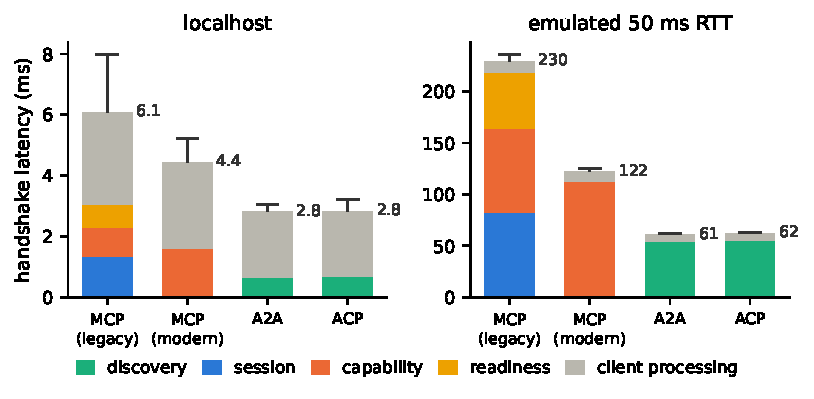
\includegraphics[width=\textwidth]{figures/f2_phase_latency.pdf}
\caption{S1 handshake latency decomposed by phase (median stacked, whisker
to p95 of the total). Note the differing y-scales: on loopback the cost is
client processing; at 50\,ms RTT the wire phases dominate in proportion to
their round trips.}
\label{fig:phase}
\end{figure}

\paragraph{The cost is round trips, not bytes or compute.}
The phase decomposition (Figure~\ref{fig:phase}) locates it. On loopback
most of every handshake is client processing: SDK object construction, JSON
parsing, validation. At 50\,ms RTT the picture inverts, and each phase's
share tracks its round trips. Sweeping emulated RTT makes the mechanism
direct: latency rises linearly with fitted slopes of \SlopeAtoa{} (A2A),
\SlopeAcp{} (ACP), \SlopeMcpModern{} (\mcpm{}), and \SlopeMcpLegacy{}
(\mcpl{}) milliseconds per millisecond of RTT. The single-fetch protocols
track their one round trip almost exactly; the legacy slope reflects three
delayed requests plus five delayed response chunks, or four RTT
equivalents. Wire volume tells a consistent but secondary story:
\SOneMcpLegacyLocalBytesUp{}+\SOneMcpLegacyLocalBytesDown{}\,B for \mcpl{}
against \SOneAtoaLocalBytesUp{}+\SOneAtoaLocalBytesDown{}\,B for A2A, a
difference invisible next to the round-trip effect at interactive
timescales.

\paragraph{Warm reconnection separates the protocols more than cold start.}
\mcpl{} can skip nothing: its specification predates response caching, so a
reconnecting client repeats all three round trips
(\STwoMcpLegacyWarmRttMed{}\,ms at 50\,ms RTT, within noise of its cold
handshake). \mcpm{} under the SDK's default policy re-probes but serves the
tool list from the SEP-2549 cache (\STwoMcpModernWarmRttMed{}\,ms). A
client that additionally pins the counterpart's protocol era reaches
task-ready with zero wire exchanges in \STwoMcpPinnedWarmRttMed{}\,ms, the
same regime as A2A's cached card (\STwoAtoaWarmRttMed{}\,ms) and ACP's
cached manifest (\STwoAcpWarmRttMed{}\,ms). Over $k{=}100$ interactions
with the same counterpart the per-interaction cost amortises to
\AmortMcpLegacy{}\,ms for \mcpl{}, effectively unamortised, against
\AmortAtoa{}\,ms for A2A. For agent pairs that interact repeatedly,
cacheability rather than cold-start cost is the design property that
matters; for true strangers, the cold numbers stand.

\paragraph{Rejection costs as much as acceptance.}
Time-to-rejection mirrors time-to-ready, because in all three protocols the
initiator discovers what a counterpart \emph{cannot} do the same way it
discovers what it can. A2A and ACP reject after their single metadata fetch
(\SThreeAtoaRttMed{} and \SThreeAcpRttMed{}\,ms at 50\,ms RTT), while
\mcpl{} must complete its entire three-round-trip handshake, session
included, before learning the counterpart is useless to it
(\SThreeMcpLegacyRttMed{}\,ms). Document-centric discovery makes ruling a
counterpart out as cheap as one GET; session-first designs charge the
session price merely to browse, which compounds for agents that shop across
many counterparts.

\paragraph{Only MCP validates version claims during the handshake.}
Both MCP eras refuse a counterpart advertising only a fictitious version in
\SFourCMcpLegacyLocalTtfMed{}--\SFourCMcpModernLocalTtfMed{}\,ms with an
explicit error, the modern probe's structured error even carrying the
server's supported-version list. A2A's client instead fetched a card
claiming protocol version 99.0.0, selected a binding, and completed tasks
without warning. This is spec-conformant, not an SDK bug: the normative
schema marks the interface's \code{protocolVersion} as descriptive, and
A2A's mandatory negotiation happens per request via an \code{A2A-Version}
header the server must reject when unsupported~\citep{a2aspec2026}. On the
wire we observed exactly that split, the client sending its own version
independent of the card's claim. The consequence for handshake design
stands: discovery-time version claims go unvalidated, so a real
incompatibility surfaces at the first task message rather than during the
handshake, and never at all when the wire versions happen to agree. ACP has
no version field to check. All protocols detect truncated metadata quickly
and abort rather than degrade (Appendix~\ref{app:degraded}).

\begin{table}[t]
\centering
\tabfont
\caption{Handshake metadata in tokens as the counterpart's capability
inventory grows, and the marginal cost of one capability. Built by
replicating the captured wire entry $n$ times inside the byte-identical
envelope, so these are the documents an $n$-capability counterpart serves.}
\label{tab:inventory}
\begin{tabular}{lrrrrr}
\toprule
Protocol & $n{=}1$ & $n{=}10$ & $n{=}50$ & $n{=}200$ & per cap. \\
\midrule
MCP & 96 & 798 & 3,918 & 15,618 & 78 \\
A2A & 115 & 331 & 1,291 & 4,891 & 24 \\
ACP & 112 & 1,075 & 5,355 & 21,405 & 107 \\
\bottomrule
\end{tabular}
\end{table}

\paragraph{Context, not dollars, is the scarce resource.}
When the initiator is an LLM the counterpart's metadata is not merely
transferred but \emph{read}, placed in a context window to select a tool or
validate a counterpart. For a one-capability counterpart the cost is
trivial, \TokAcp{}--\TokMcpModern{} tokens, and should be treated as a
protocol floor rather than a cost. The slope is the finding
(Table~\ref{tab:inventory}). Each additional capability costs
\InvPerCapAtoa{} tokens in an A2A card, \InvPerCapMcp{} in an MCP tool
listing, and \InvPerCapAcp{} in an ACP manifest. At \InvMaxN{} capabilities
the handshake alone delivers \InvMcpNTwoHundred{} tokens for MCP and
\InvAcpNTwoHundred{} for ACP, which is \InvMaxCtxPct{}\% of a 200k-token
window spent before the agent reads its own task.

The per-capability costs differ by more than a factor of four, and the
ordering inverts against the one-capability ranking: A2A is cheapest
because a skill entry is a name, a description, and tags, MCP dearer
because a tool entry carries full input and output JSON schemas, ACP
dearest because each agent entry repeats a sixteen-field metadata block. A
protocol's floor says little about what it costs at deployment scale. This
is also the one handshake cost that round-trip reduction does not touch: it
is carried by the listing step, which every protocol performs and which the
2026 MCP revision made cacheable but no cheaper.

\section{Discussion}
\label{sec:discussion}

Handshake cost is round trips first, connections second, bytes a distant
third, and compute negligible. Every design question about agent handshakes
should therefore be asked as ``how many round trips does this add, and can
it be cached?'' The protocols' own trajectories agree: MCP's 2026 revision
is precisely a round-trip-reduction release, replacing a three-message
session-first initialisation with a one-probe cacheable discovery, and our
measurements quantify the effect at \McpModernSpeedup{}\% off the cold
handshake at 50\,ms RTT. That the youngest protocol in our study already
shipped this change is evidence that handshake overhead is a live design
pressure rather than a hypothetical.

For an OS layer over agentic systems, three implications follow directly.
Treat counterpart metadata as a cacheable asset with a lifecycle, since the
measured gap between \mcpl{} and everything else is mostly the gap between
re-deriving and reusing handshake state. Budget round trips at discovery
time when an agent shops across many counterparts, because rejection costs
a full handshake and a design that rules counterparts out from one GET
scales shopping linearly rather than in handshakes. And treat the context
window as a first-class budget: the per-capability slope, not the floor, is
what binds, and it is the cost caching defers but round-trip reduction
never removes.

The measurements have real limits. Our counterparts expose one capability,
so latency figures are protocol floors, which is why we sweep inventory
size for the metadata costs. Emulation is userspace rather than kernel
level, so transport setup is excluded from the RTT figures, and we quantify
the direction of that bias rather than claim it away. We measure specific
SDK versions at a specific date, and SDK-added behaviour is part of what we
measure deliberately, because it is what deployed agents actually pay.
Authenticated handshakes and live natural-language negotiation are the
obvious next cells; both add round trips and tokens that deserve the same
decomposition.

\bibliographystyle{plainnat}
\bibliography{refs}

\appendix

\section{Threats to Validity}
\label{app:validity}

\emph{Toy counterparts.} Our agents expose one capability. Real
counterparts with large inventories shift byte and token costs upward,
which is why Table~\ref{tab:inventory} sweeps inventory size directly;
handshake latency is less affected, since inventory changes payloads rather
than round trips.

\emph{Userspace network emulation.} The relay delays application-layer
chunks, not packets. TCP establishment against it completes at loopback
speed, so the 50\,ms-RTT figures exclude transport setup entirely; on a
real 50\,ms link each connection would add one RTT, plus one for TLS~1.3,
which penalises exactly the protocols that open more connections. SSE
responses cross in two chunks and pay the per-chunk delay twice, which
parallels but does not perfectly model per-packet kernel emulation. Both
biases run against the protocol we report as cheapest, so the measured gap
is conservative. Reproducing these cells under kernel-level emulation is
the first thing we would add.

\emph{Single SDK generation, single machine.} We measure specific SDK
versions on one Apple-silicon machine over loopback. Round-trip and byte
counts, which drive the higher-RTT results, are machine-independent;
absolute low-RTT latencies are not.

\emph{Token accounting.} Token counts use an open tokenizer as a lower
bound; a frontier vendor's tokenizer counts roughly 15--20\% higher on
JSON-like content. Byte counts are exact.

\section{Degraded Conditions in Full}
\label{app:degraded}

\begin{table}[h]
\centering
\tabfont
\caption{Behaviour under degraded conditions ($N{=}\NRuns{}$ per cell,
localhost). S4a reports time to task-ready with a 2\,s per-response server
delay; S4b and S4c report time to failure. For S4c, ACP is untestable: its
manifest carries no protocol-version field.}
\label{tab:degraded}
\begin{tabular}{llllrl}
\toprule
Scenario & Protocol & Outcome & med.\ time (ms) & Retr. & Error surfaced \\
\midrule
S4a slow (2\,s/resp.) & MCP (legacy) & ready & 6026 & 0 & none \\
 & MCP (modern) & ready & 4019 & 0 & none \\
 & A2A & ready & 2011 & 0 & none \\
 & ACP & ready & 2011 & 0 & none \\
\addlinespace
S4b truncated metadata & MCP (legacy) & error & 3.5 & 0 & \texttt{MCPError} \\
 & MCP (modern) & error & 4.4 & 0 & \texttt{MCPError} \\
 & A2A & error & 3.0 & 0 & \texttt{AgentCardResolutionError} \\
 & ACP & error & 2.9 & 0 & \texttt{JSONDecodeError} \\
\addlinespace
S4c version mismatch & MCP (legacy) & error & 3.7 & 0 & \texttt{RuntimeError} \\
 & MCP (modern) & error & 4.2 & 0 & \texttt{RuntimeError} \\
 & A2A & ready & 3.0 & 0 & none (version deferred) \\
\bottomrule
\end{tabular}
\end{table}

With 2\,s injected per response, time to task-ready is a clean multiple of
round-trip count: \SFourAMcpLegacyLocalMed{}\,ms for \mcpl{} against about
2\,s for A2A and ACP. No SDK timed out or retried; the delay simply
multiplies, so a slow counterpart is most expensive to the protocol with
the most round trips, and the initiator cannot discover the slowness before
paying the full handshake.

Against metadata truncated at 50\%, all four variants fail fast, with no
retry storms and no hangs, every client detecting invalid JSON on first
parse in milliseconds. What differs is error quality. A2A names the
offending URL and MCP reports a protocol-level validation failure, while
ACP surfaces a bare \code{JSONDecodeError} with a character offset and no
indication of which endpoint or agent was involved. All three abort rather
than degrade, which is right; only ACP leaves the caller to reconstruct the
context. For autonomous agents, which cannot eyeball a stack trace, the
difference between a structured ``unsupported version, here is what I
support'' and a counterpart whose incompatibility surfaces only at task
time is the difference between a recoverable negotiation and a debugging
session.

\section{Transport-Layer Baseline}
\label{app:baseline}

For calibration, on the same loopback a bare TCP connect completes in
\BaselineTcpMed{}\,ms and a full TLS~1.3 handshake in \BaselineTlsMed{}\,ms
of compute, one round trip each on a real network~\citep{rescorla2018tls}.
Against that two-round-trip transport-plus-cryptographic stack, A2A and ACP
add a single application-layer round trip, half the cost of the stack
beneath them, while a legacy MCP handshake adds three, exceeding the
combined transport and cryptographic setup it rides on, before any
authentication. The application layer has in effect re-created the
pre-TLS-1.3 handshake stack one level up, and is now re-learning the same
remedies, fewer round trips and resumable state, that transport designers
adopted a decade ago~\citep{lee2021tls,iyengar2021quic}.

\section{Reproducibility}
\label{app:repro}

The released repository contains the harness, minimal counterpart agents,
raw per-run JSONL for every cell in this paper, and the analysis scripts
that generate every figure, table, and in-text number. Three commands
reproduce the raw data and one regenerates every artifact from it; the
first takes roughly 25 minutes on a laptop. Version pins: Python 3.12.13,
\code{mcp} 2.0.0, \code{a2a-sdk} 1.1.2, \code{acp-sdk} 1.0.3, \code{httpx}
0.28.1, \code{uvicorn} 0.34.3, \code{fastapi} 0.115.14, \code{starlette}
0.46.2. The MCP counterpart is served over streamable HTTP with SEP-2549
cache hints (one hour, public scope) on \code{server/discover} and
\code{tools/list}; the A2A counterpart serves a v1.0 Agent Card with one
skill over the JSON-RPC binding; the ACP counterpart serves one agent
manifest. Repository URL withheld for double-blind review. ANONYMISED.

\end{document}
